\newcommand{\lavKolonneData}[3]{  
    % Store in the column variables (c1, c2, c3,...)
    \expandafter\xdef\csname c1\the\numexpr\value{raekketaeller}+1\endcsname{#1}  
    \expandafter\xdef\csname c2\the\numexpr\value{raekketaeller}+1\endcsname{#2}  
    \expandafter\xdef\csname c3\the\numexpr\value{raekketaeller}+1\endcsname{#3}  
    
    % Increment the column counter for the next column
    \stepcounter{raekketaeller}  
}
% Set up a counter to keep track of the column number
\newcounter{raekketaeller}\setcounter{raekketaeller}{0}


\NewDocumentEnvironment{EgenTabel}{+b}{
    % ------- Lav dataen -------
    #1 
}{
    % ------- Vis dataen -------
    \vspace{10pt}
    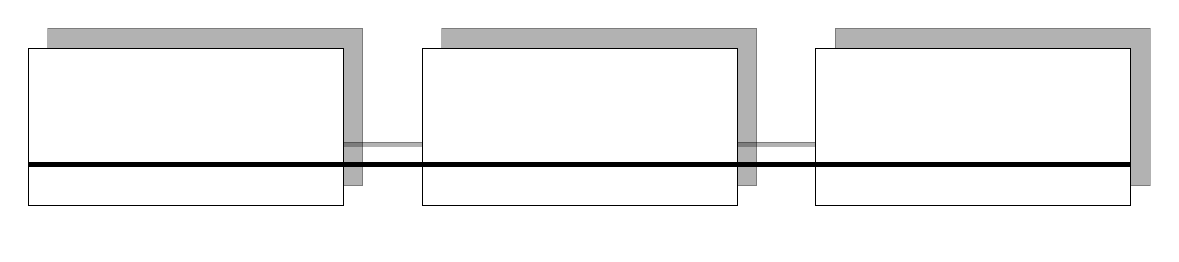
\begin{tikzpicture}
        \tikzset{
            shadow/.style={fill=black, opacity=0.3},        % Skygge 
            cell/.style={fill=white, draw=black, very thin}, % Celle 
        }
        % Baggrund of celler
        \filldraw[shadow] (0.25, 0.5*\theraekketaeller + 2 + 0.25 - 1.5) rectangle(12, 0.5*\theraekketaeller + 2 + 0.25 - 1.5 + 0.05);
        \foreach \x in {0, ..., 2} {
            \filldraw[shadow] (\x*5 + 0.25, 0.25) rectangle(\x*5 + 4.25, 0.5*\theraekketaeller + 2 + 0.25); 
            \filldraw[cell] (\x*5, 0) rectangle(\x*5 + 4, 0.5*\theraekketaeller + 2); 
        }
        % Visning af data.
        \foreach \i in {1, 2, ..., \theraekketaeller} {
            \ifnum\i=1
                \filldraw[black] (0.5, 0.5*\theraekketaeller + 2 - 0.75) node[anchor=west] {$\csname c1\i\endcsname$};
                \filldraw[black] (5.5, 0.5*\theraekketaeller + 2 - 0.75) node[anchor=west] {$\csname c2\i\endcsname$};                
                \filldraw[black] (10.5,0.5*\theraekketaeller + 2 - 0.75) node[anchor=west] {$\csname c3\i\endcsname$};
            \else
                \filldraw[black] (0.5, 0.5*\theraekketaeller + 2 - 1.25 - 0.5*\i) node[anchor=west]{$\csname c1\i\endcsname$};
                \filldraw[black] (5.5, 0.5*\theraekketaeller + 2 - 1.25 - 0.5*\i) node[anchor=west]{$\csname c2\i\endcsname$};
                \filldraw[black] (10.5, 0.5*\theraekketaeller + 2 - 1.25 - 0.5*\i) node[anchor=west]{$\csname c3\i\endcsname$};
            \fi
        }
        % Horinsontal linje. 
        \filldraw[black] (0, 0.5*\theraekketaeller + 2 - 1.5) rectangle(14, 0.5*\theraekketaeller + 2 - 1.5 + 0.05);
    \end{tikzpicture}\setcounter{raekketaeller}{0}
}






